\documentclass[conference]{IEEEtran}
\IEEEoverridecommandlockouts
% The preceding line is only needed to identify funding in the first footnote. If that is unneeded, please comment it out.
\usepackage{cite}
\usepackage{amsmath,amssymb,amsfonts}
\usepackage{algorithmic}
\usepackage{graphicx}
\usepackage{textcomp}
\usepackage{xcolor}
\def\BibTeX{{\rm B\kern-.05em{\sc i\kern-.025em b}\kern-.08em
    T\kern-.1667em\lower.7ex\hbox{E}\kern-.125emX}}
\begin{document}

\title{MetaKicks\\{\Large
 Virtual LG Styler ShoeCase with real-time price tracking 
 }
}

\author{\IEEEauthorblockN{Kwon Jihyun 2018007383}
\IEEEauthorblockA{\textit{College of engineering,} \\
\textit{Hanyang University}\\
\textit{Dept. of Information system}\\
Seoul, Korea \\
nahoo0705@hanyang.ac.kr}
\and
\IEEEauthorblockN{Kim Younghwan 2018007410}
\IEEEauthorblockA{\textit{College of engineering,} \\
\textit{Hanyang University}\\
\textit{Dept. of Information system}\\
Seoul, Korea \\
wizde20@hanyang.ac.kr}
\and
\IEEEauthorblockN{Lee Jiyun 2018007692}
\IEEEauthorblockA{\textit{College of engineering,} \\
\textit{Hanyang University}\\
\textit{Dept. of Information system}\\
Seoul, Korea \\
dlwldbs9764@hanyang.ac.kr}
\and
\IEEEauthorblockN{Jeong Youngho 2018007765}
\IEEEauthorblockA{\textit{College of engineering,} \\
\textit{Hanyang University}\\
\textit{Dept. of Information system}\\
Seoul, Korea \\
zer0kola321@hanyang.ac.kr}
}

\maketitle

\begin{abstract}
\textit{As the culture of collecting expensive designer, luxury and limited-edition sneakers grows among the MZ generation – Millennials and Gen Z – LG’s internal research found that these ‘sneakerheads’ would benefit greatly from a solution that not only made their cherished shoes stand out more, but also provided them with the optimal care. So LG has launched the LG Styler ShoeCase, which not only optimizes shoe management but also increases the value of collection and provides LG ThinQ applications to connect its home appliances and consumers and provide consumers with a better experience. So our team thought that it would be good to virtualize the ShoeCase and manage it on this project. NFT sneakers that exist only virtually are collected as if it were stored in a LG Styler ShoeCase with MetaKicks project. In addition, the limited edition of the shoe resell market has grown a lot, and we decided to create this service to check the resale market price of shoes in real time. Finally, we thought that the culture of collecting shoes could be further activated by taking out the shoe case that was only in my room on the web and creating a culture to share each other's shoes collections.}\end{abstract}

\begin{table}[h]
\caption{Role Assignments}
\def\arraystretch{1.24} \small
    \begin{tabular}{|p{1.8cm}|p{1.4cm}|p{4.4cm}|}
        \hline
        Roles & Name & Task description and etc. \\ \hline
         User \par Customer & Kwon \par Jihyun & User/Customer contemplates what functions should be added from the perspective of users or customers. For example, the 'MetaKicks' has a function of realtime price tracking in addition to simply adding shoes in virtual ShoeCase. and provides the ability to share each other's collections.\\ \hline
         
          Product \par Designer& Kim \par Younghwan  & A product designer is a person with user-centered thinking ability to sympathize with and understand the user's experiences and plays a role in creating an overall framework for product and services. It performs smooth collaboration with other team members with  excellent communication skills. It focuses on the usability of products and services and performs designs to provide better results.\\ \hline
 
	\end{tabular}
\end{table}

\begin{table}
\def\arraystretch{1.24} \small
    \begin{tabular}{|p{1.8cm}|p{1.4cm}|p{4.4cm}|}
        \hline
              
        Software \par Developer & Jeong \par Youngho  & A software developer refers to a person who makes software. This includes discovering a meaningful service and accurately grasping the needs of a user who wants to use the service. In addition, there is a need for the ability to design and code these services and user needs in software. Furthermore, the software developer tests the created program. \\ \hline
        
        Development \par manager & Lee \par Jiyun & Development Manager manages the overall part of the project, such as the schedule/planning of the project and the quality of products and services. It also manages/supervises the entire software engineering process of designing, developing, and testing software from accurately grasping user  requirements. In addition, in this process, Development Manager helps project participants communicate smoothly. \\ \hline
    \end{tabular}
\end{table}

\section{Introduction}
\subsection{Motivation}
Shoe cases so far are made of plastic and can only function as storage and display shoes. But The LG Styler ShoeCase creates the ideal environment for storing shoes by protecting against humidity and fabric-discoloring UV light, the Styler ShoeCase represents a great way for shoe enthusiasts to show-off their favorite pairs, offering interior features such as a 360-degree rotating turntable to increase the value as a collection rather than just shoes. 
NFT shoes are stored online, and real shoes are stored only in the ShoeCase and managed separately. By using this, these two collections are managed by one app. We thought it would be good to share the collection, including NFT shoes, with various people to further boost the shoe collection culture.
So we make this service by paying attention to the value of the collection. It check the fluctuating resell market price in real time using Kream or StockX's API, Korea and USA's leading sneakers trade site, and sharing each other's collections through this service.


\subsection{problem statement}
\begin{itemize}
\item In The case of limited-edition shoes, prices fluctuate significantly over time or depending on events, so collectors who own several shoes find it difficult to know the value of the collections at once.
\item The shoe case so far is just a plastic drawer. There is only a storage function and the function of the exhibition is inferior. There are many people who want to manage it like a proper collection.
\item NFT shoes can only be stored online or on a hard disk, and real shoes are in ShoeCase, so there is no means to manage both at once
\item It is very useful to use a LG Styler ShoeCase to manage sneakers. but there is no means to check the shoes stored at home outside.
\item You can't see other people's sneakers collection unless you go their home. In order for the shoe collection community to grow further, it is necessary to have the ability to see collections of many people
\end{itemize}

\subsection{Research of any relative software}

{Kream} \\ It is a transaction brokerage platform that connects sellers and buyers anonymously. Similar to trading methods such as stocks and cryptocurrencies, it consists of presenting the price the seller wants to sell and accepting the price. Due to the nature of the asking price transaction, used goods are not handled because the premise that all items are the same is necessary. The main trading items are limited edition products such as clothing and fashion miscellaneous goods, and can be seen as a commonly referred to as a resale trading platform. Unlike general direct transaction platforms, products are traded through the KREAM inspection center. When the seller sends the product to the KREAM inspection center, the KREAM inspects it and sends it to the buyer.\\

{StockX} \\ It serves as an online marketplace, facilitating auctions between sellers and buyers, then collecting transaction and payment fees. Sellers send purchased items to StockX facilities for inspection and verification, then authenticated products are shipped to buyers. StockX features a "stock market-like" variable pricing framework and discloses price histories for specific items. StockX is most known for sneakers and streetwear but also carries other clothing and accessories such as handbags and watches.\\

{LG ThinQ} \\ A representative home appliance management app that provides smart home services based on AI. With this application, you can control not only home appliances, but also all parts of the house, as well as check product status and malfunctions anytime, anywhere. In a situation in which the market environment is rapidly changing from 'supplier-centered' to 'consumer-centered, LG is providing these services, believing that the role of AI technology has grown.\\

\section{Requirement Analysis}

\subsection{Login}
It supports Google login and Apple login by linking Firebase and React. If the login is successful, you will be taken to the main page.\\

\subsection{Main Page}
Users can check the functions in the app at once on the main page. \\
\begin{enumerate}
    \item My ShoeCase\\
    \item Finding Other User\\
    \item Favorite ShoeCase\\
\end{enumerate}

\subsection{My ShoeCase}
My ShoeCase page visualizes LG Styler ShoeCase on the LG thinQ app. There is no Shoes in the first entry. There is a pop-up page that writes the name or serial number of the ShoeCase product, then a virtual ShoeCases will be created according to the number of rooms and size of the ShoeCase. A user can nickname the user's ShoeCase.
\\
\begin{enumerate}
    \item Register Shoes by Style Code: There is a button for registering shoes in each section of the ShoeCase. When the user clicks the button, a pop-up window appears, and the user can search style code on the shoes site and register the shoes. For NFT shoes, there is an NFT shoe registration button. When you click the button, a pop-up window appears, and if you enter NFT information for the shoes, you will be registered in the virtual shoe closet like normal shoes.
\\
    \item Registered Shoes Information: The name and real-time resell price of the shoes displayed on the virtual ShoeCase. When the user clicks the shoes, The product’s site will appear to show the information of shoes linking with the shoes site.
\\
    \item Public/Private Setting: There is a checkbox to determine to show the user's ShoeCase
\\
    \item The number of Kick: Those who have seen user's ShoeCase and like it press the Kick. Total number of Kicks is displayed.
\\
\end{enumerate}

\subsection{Finding Other User}

Other people's ShoeCase is listed only for those allowed to reveal their ShoeCase. The list displays the user's name and the nickname of the ShoeCase. When the user clicks the name of the person the user wants to see, the page switches to the that person's ShoeCase page.
\\
\begin{enumerate}
	\item Search Someone's ShoeCase: You can search the user's nickname and view the published ShoeCase.
\\
	\item Recommendation: List ShoeCase by number of Kicks. 
\\
\end{enumerate}

\subsection{Favorite ShoeCase}

There is no ShoeCases in the first entry. If you click the Kick button on your favorite ShoeCase among other people's ShoeCase. The ShoeCases are registered in my favorites. And Click the ShoeCase button to go to the user's ShoeCase. Sends a notification whenever new shoes are added to your favorite ShoeCase. 
\\
\begin{enumerate}
	\item Favorite ShoeCase lists: List your favorite ShoeCases.
	\\
	\item Visit Someone's ShoeCase: If you click the ShoeCase's nickname on the list, app shows that user's ShoeCase Page. 
\\
\end{enumerate}

\section{DEVELOPMENT ENVIRONMENT}

\subsection{Software development platform}
The development environment we chose is Windows and Mac. We developed it according to the operating system of each laptop, and built and operated the source code using the terminal functions of Windows and Mac. The front-end framework chose react-native and nodejs as the back-end development language. React-native is a cross-platform framework that can be developed simultaneously on Android and iOS operating systems, and it is the most popular front-end framework, so I chose it in the hope that it will be studied while working on the project. Nodejs is a run-time environment that allows you to run code that builds servers outside your browser based on JavaScript language, making it easy to expand servers and highly compatible with react-native, so we chose it as a back-end development language.\\
\begin{table}[h]
\caption{Develop Environment}
\def\arraystretch{1.25} \small
    \begin{tabular}{|p{2.4cm}|p{5.0cm}|}
	\hline
	Name & Development Environment\\
       \hline
       Kwon Jihyun & Windows10 21H2, VScode 1.72.2, node.js 18.12.0 \\
	\hline
        Kim Younghwan & Windows10 21H2, VScode 1.72.2, node.js 18.12.0\\
	\hline
	\end{tabular}
\end{table}
\begin{table}
\def\arraystretch{1.25} \small
    \begin{tabular}{|p{2.4cm}|p{5.0cm}|}
	\hline
        Lee Jiyun & Windows10 21H2, VScode 1.72.2, node.js 18.12.0\\
	\hline
	Jeong Youngho & MacOS Monterey 12.6, VScode 1.72.2, node.js 18.12.0\\
	\hline
	\end{tabular}
\end{table}

\begin{table}[h]
\caption{Platform, Programming Language, Database}
\def\arraystretch{1.25} \small
    \begin{tabular}{|p{2.4cm}|p{5.0cm}|}
	\hline
	Tools and Language & Reason\\
      \hline
       Javascript & JavaScript is one of the most popular web development programming languages. It is one of the components of the web today, along with HTML and CSS. Javascript can handle not only the front-end but also the back-end. Javascript is the basic programming language for React and Node.js. With one programming language, we can care for each other and review. Javascript is easy and fast to manage posts posted in real time. \\
	\hline
        MongoDB & MongoDB is a NoSQL database that stores data as JSON-like documents. MongoDB enables us to build applications faster than sql, handle highly diverse data types, and manage applications more efficiently at scale. MongoDB is also easy to process vast amounts of data. Metakicks will handle the data of many user's shoecase, handling a large amount of data is required.\\
	\hline
        Node.js & Node.js is a software platform used to develop scalable network applications. Node.js utilizes JavaScript as the writing language and has high processing performance through non-blocking I/O and single thread event loops. Node.js has the ease of server expansion and can even write back-end in the required front-end language of JavaScript. Also Node.js has a strong point in services that require processing a huge amount of input output data.\\
	\hline
	React-Native & React native is a framework for developing Android and iOS apps using React's grammar. React native also uses Javascript as a programming language, so it has good versatility. Hot Reload and Live Reload of React native allows us to immediately apply the correction and confirm the correction immediately.\\
	\hline
	\end{tabular}
\end{table}

\subsection{Software in use}
\begin{enumerate}
	\item{KREAM}\\
	\\
	\centerline{
\includegraphics[scale=0.2]{pics/KREAM.png}}\\\\
It is a transaction brokerage platform that connects sellers and buyers anonymously. Similar to trading methods such as stocks and cryptocurrencies, it consists of presenting the price the seller wants to sell and accepting the price. Due to the nature of the asking price transaction, used goods are not handled because the premise that all items are the same is necessary. The main trading items are limited edition products such as clothing and fashion miscellaneous goods, and can be seen as a commonly referred to as a resale trading platform. Unlike general direct transaction platforms, products are traded through the KREAM inspection center. When the seller sends the product to the KREAM inspection center, the KREAM inspects it and sends it to the buyer.\\
	\item{StockX}\\
	\\
	\centerline{
\includegraphics[scale=0.2]{pics/StockX.png}}\\\\
StockX serves as an online marketplace, facilitating auctions between sellers and buyers, then collecting transaction and payment fees. Sellers send purchased items to StockX facilities for inspection and verification, then authenticated products are shipped to buyers. StockX features a "stock market-like" variable pricing framework and discloses price histories for specific items. StockX is most known for sneakers and streetwear but also carries other clothing and accessories such as handbags and watches.\\
	\item{LG ThinQ}\\
	\\
	\centerline{
\includegraphics[scale=0.4]{pics/LG.png}}\\\\
A representative home appliance management app that provides smart home services based on AI. With this application, you can control not only home appliances, but also all parts of the house, as well as check product status and malfunctions anytime, anywhere. In a situation in which the market environment is rapidly changing from 'supplier-centered' to 'consumer-centered, LG is providing these services, believing that the role of AI technology has grown.\\
	\item{GitHub}\\
	\\
	\centerline{
\includegraphics[scale=0.4]{pics/GitHub.png}}\\\\
It is a representative free git platform, and a small platform between teams. In Mark-down language, you can create the above key in Mark-down language, and highlight the important content. Through all documents and functions of the project, it improved work ability to share all documents and functionality. We will also use the branch function to complete the coding of each part and combine it if there is no problem.We will use github to share works with each other and proceed with development gradually. Development documents are also periodically attached in latex file format.\\
	\item{node.js}\\
	\\
	\centerline{
\includegraphics[scale=0.13]{pics/nodejs.png}}\\\\
Node.js is an open-source, cross-platform, back-end JavaScript runtime environment that runs on a JavaScript Engine (i.e. V8 engine) and executes JavaScript code outside a web browser, which was designed to build scalable network applications. Node.js lets developers use JavaScript to write command line tools and for server-side scripting—running scripts server-side to produce dynamic web page content before the page is sent to the user's web browser.We adopted Node.js as a backend system for developing applications. As for the front end, Node.js was considered suitable because React Native was selected in consideration of the interworking of JavaScript instead of flutter.\\
	\item{React-Native}\\
	\\
	\centerline{
\includegraphics[scale=0.4]{pics/React-Native.png}}\\\\
React Native is an open-source UI software framework created by Meta Platforms, Inc. It is used to develop applications for Android, Android TV, iOS, macOS, tvOS, Web, Windows and UWP by enabling developers to use the React framework along with native platform capabilities. We adopted reactive native as a front-end system for developing applications. As for the backend, Node.js was selected instead of flask in consideration of the interworking of JavaScript, so I thought react native would be suitable.\\
	\item{VScode}\\
	\\
	\centerline{
\includegraphics[scale=0.05]{pics/VScode.png}}\\\\
Visual Studio Code is a source code editor developed by Microsoft for Windows, Linux, and macOS. It can be used with various programming languages such as Java, JavaScript, Go, Node.js, Python, C++, C, Rust, and Fortran.Features include debugging, syntax emphasis, intelligent code completion, snippet, code refactoring, and embedded Git support. Users can install extensions that change themes, keyboard shortcuts, preferences, and add additional features. VScode can utilize various languages, and we chose to take advantage of these VScode advantages.\\
	\item{Firebase}\\
	\\
	\centerline{
\includegraphics[scale=0.4]{pics/Firebase.png}}\\\\
Firebase is a back-end service that provides essential functions for the web and mobile development environment, and plays a variety of roles, including authentication functions that make Google account functions easy and Firestore functions that enable database functions. In this project, we mainly used the authentication function to facilitate the implementation of the Google login function.\\
	\item{mongoDB}\\
	\\
	\centerline{
\includegraphics[scale=0.4]{pics/mongo.png}}\\\\
MongoDB supports field, range query, and regular-expression searches. Queries can return specific fields of documents and also include user-defined JavaScript functions. Queries can also be configured to return a random sample of results of a given size. We will link the backend system Node.js with MongoDB. Among Nosql DBs, which can be said to be efficient when used with node.js, we intend to use Mongo DB, which is the most widely known.\\
	\item{Express.js}\\
	\\
	\centerline{
\includegraphics[scale=0.4]{pics/express.png}}\\\\
Express.js is a web framework based on the core modules of Node.js, http and Connect components. Express.js helps developers quickly and easily develop with Node.js. Middleware with various functions written in JavaScript code can be used by combining Express with only what developers need. We use express.js as a standard server framework. With express.js, we connect mongoDB and handle the database.
\end{enumerate}

\subsection{Cost estimation}
\begin{table}[h]
\caption{Price of Tools}
\def\arraystretch{1.25} \small
    \begin{tabular}{|p{2.4cm}|p{5.0cm}|}
	\hline
	Tools & Price\\
       \hline
       LG gram 17 & 2,019,000 * 3 = 6,057,000 won\\
	\hline
       MacBook M2 & 2,090,000 won\\
	\hline
       AWS server & 10,000 won\\
	\hline
	Total & 8,157,000 won\\
	\hline
	\end{tabular}
\end{table}
\section{Specification}

\subsection{Main Page}
\centerline{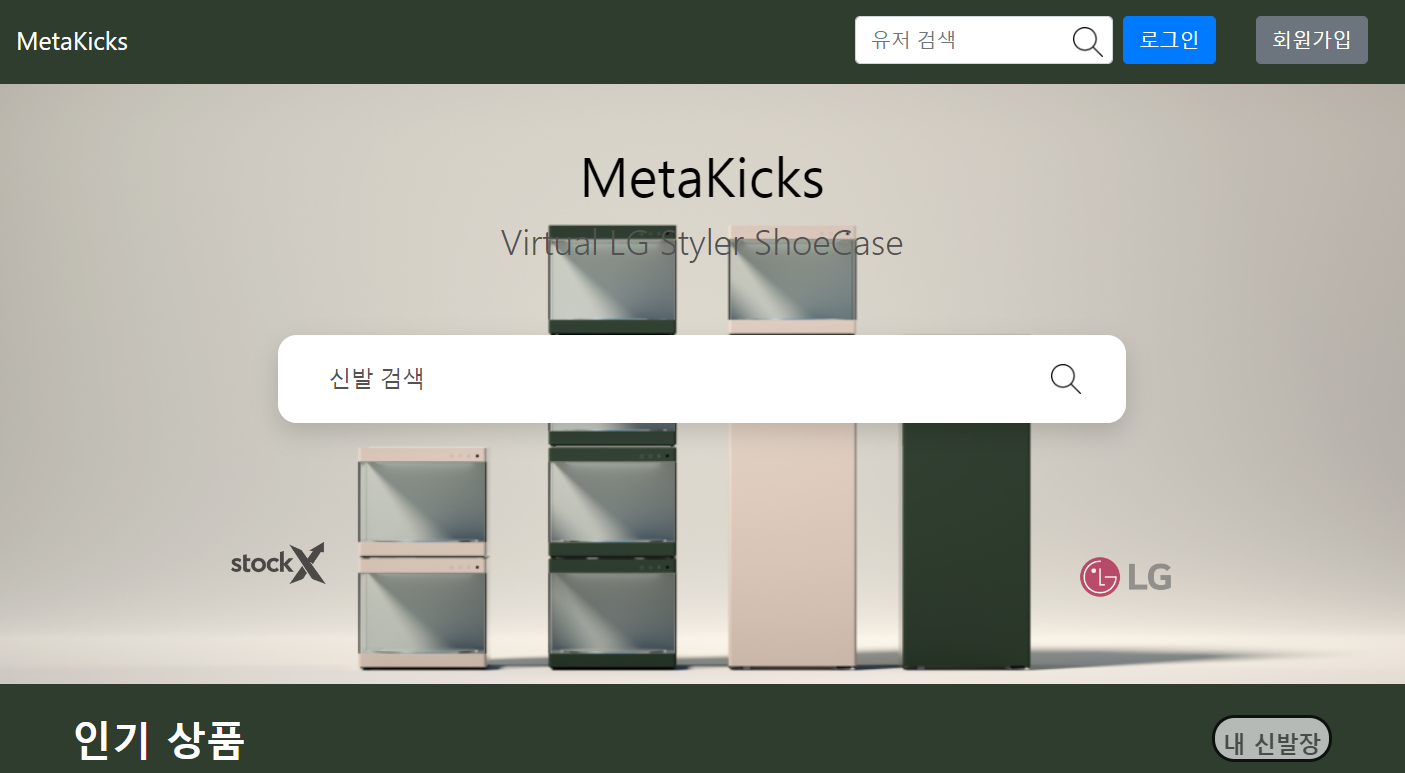
\includegraphics[scale=0.3]{pics/main_page.png}}
If you go to the Metakicks homepage, the main page appears. At the center of the main page, there is the name of  the Metakicks and at the bottom there is the search bar. On the main page, there is "Trending Now" block, which shows the current trendy products based on the stockx site. When a user presses the shoe image, a detailed description of the shoe is provided. In the upper right corner of "Trending Now", there is a button to "My ShoeCase", and when you click the button, it shows the user's shoecase. The Searchbar in the center of the page allows you to search for other shoes based on stockx data, and when you want to add the shoes to your shoecase, you can use the searchbar to find shoes and add them to your shoecase. The navigation bar at the top of the main page has buttons to login, register, search other user.\\\\
\begin{enumerate}
\item{Login}
\\\\\centerline{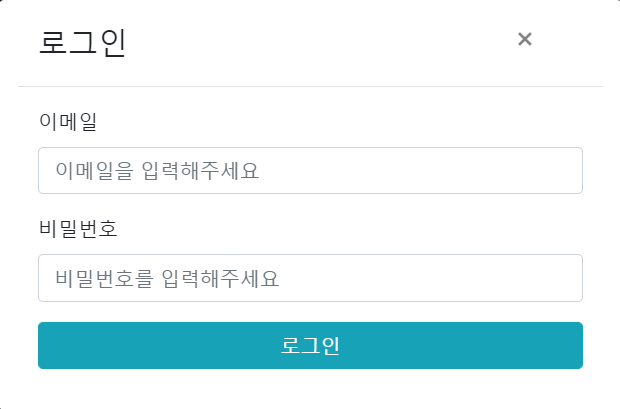
\includegraphics[scale=0.6]{pics/login.png}}
\\\\When the user presses the login button at the top of the main page, the login pop-up page appears. When the user enters the user's email and password, the login is successful.\\
\item{Login failure}\\
\\If the user failed to login Google/Apple or get error, a pop-up will appear to user. The message of the pop-up is “Error occurred while you log in. Please log in again.”. When the user clicks “confirm button”, pop-up disappear and back to login page.\\\\
\item{User Register}\\\\
\\\centerline{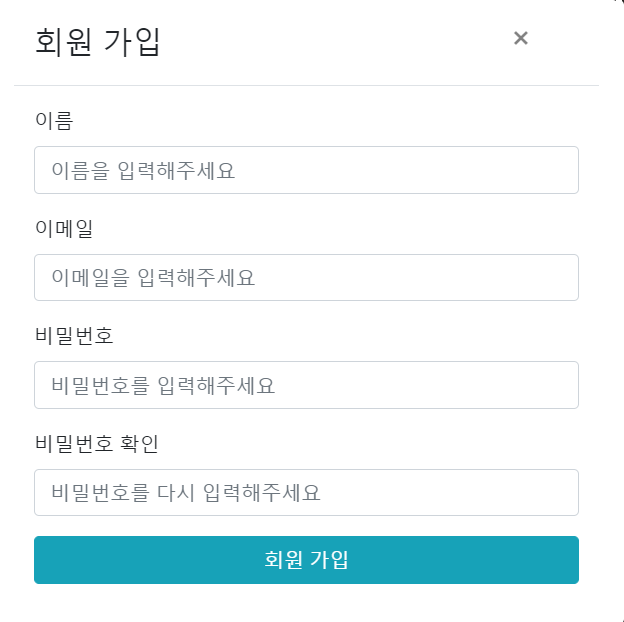
\includegraphics[scale=0.6]{pics/register.png}}\\
\\\\To sign up for the membership, Metakicks requires the user's name, email address, password and verifing password.\\
	\begin{enumerate}
		\item[-]The name must be entered in 8 characters or less.\\\\
	\end{enumerate}
	\begin{enumerate}
		\item[-]The e-mail will be exposed to the phrase asking you in follow the e-mail format and enter it.\\\\
	\end{enumerate}
	\begin{enumerate}
		\item[-]The password should be the combination of english and numbers with over 8 characters.\\\\
	\end{enumerate}
	\begin{enumerate}
		\item[-]In the password verification, the same character should be typed in this sector. If the user types the different character, registration will be denyed.\\\\
	\end{enumerate}


	\item Trending Now \\\\
\\\centerline{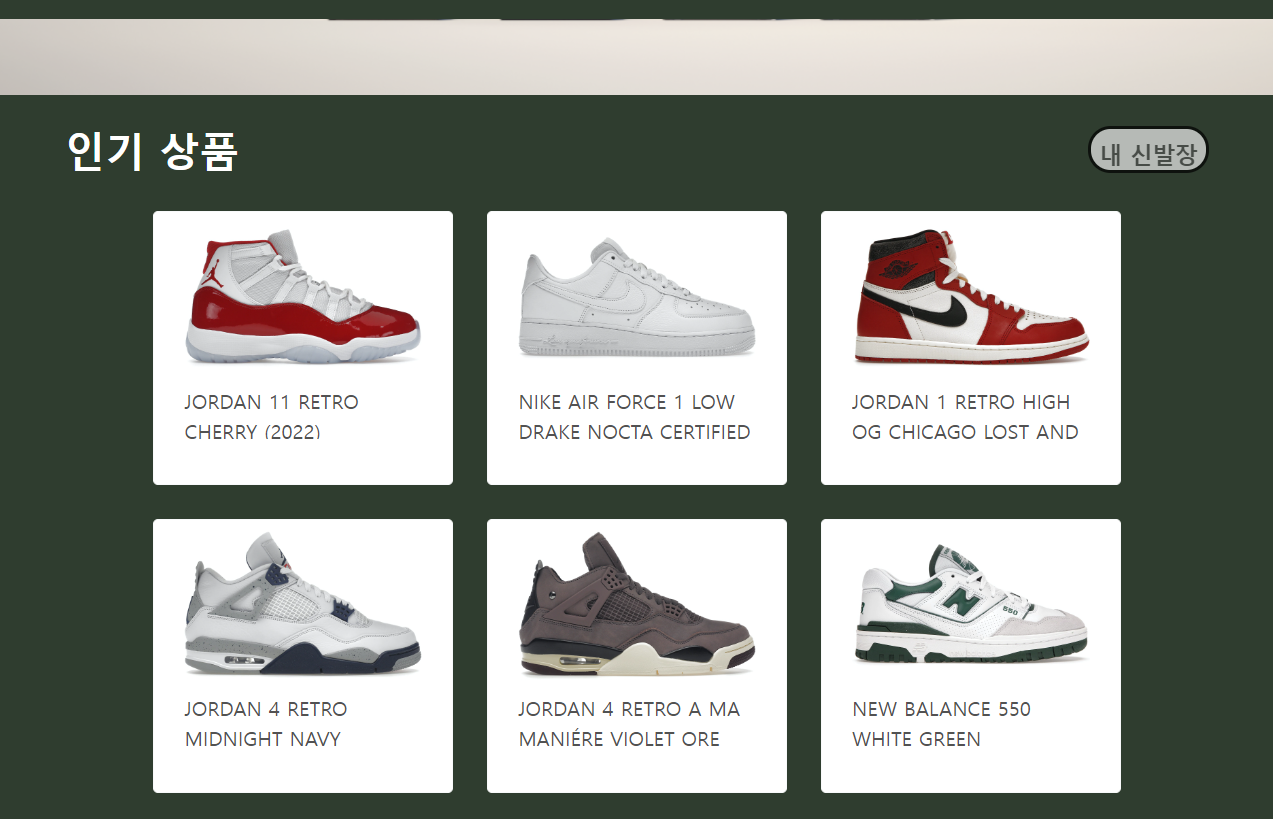
\includegraphics[scale=0.3]{pics/trending.png}}\\
\\\\ "Trending now" is organized at the bottom of the main page. "Trending now" shows the names and photos of the products currently popular on Stockx, which is the shoes trading site. If you click on a photo of the products that are on screen, a "Pop-Up" with product details appears.\\
	\item Trending Shoes Pop-Up\\\\
\\\centerline{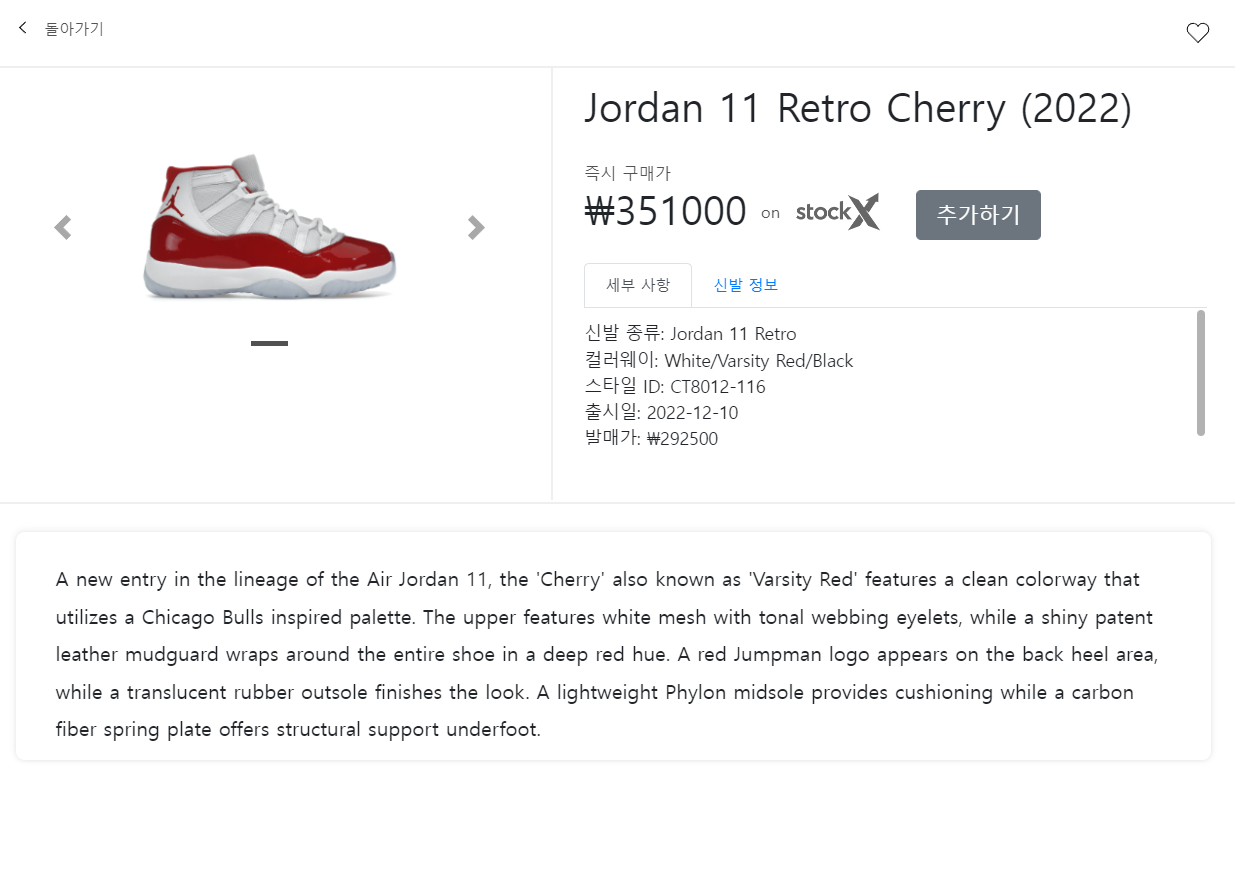
\includegraphics[scale=0.35]{pics/trending_detail.png}}
\\When the user clicks the image in "Trending now", a pop-up page appears. The pop-up contains the price of shoes and detailed information about shoes.\\\\
	\item Search Bar \\\\
\centerline{
\includegraphics[scale=0.35]{pics/searchbar.png}}\\\\
In the middle of the main page, there is a search bar. This search bar allows you to search for shoes based on stockx data. When the user enters a search word, shoes including the search word are displayed on the screen. Like "Trending Now" page, when the user clicks on an image of a shoes, a pop-up page appears with prices and details about the shoes.\\
	\item Search Shoes Pop-Up\\\\
\\\centerline{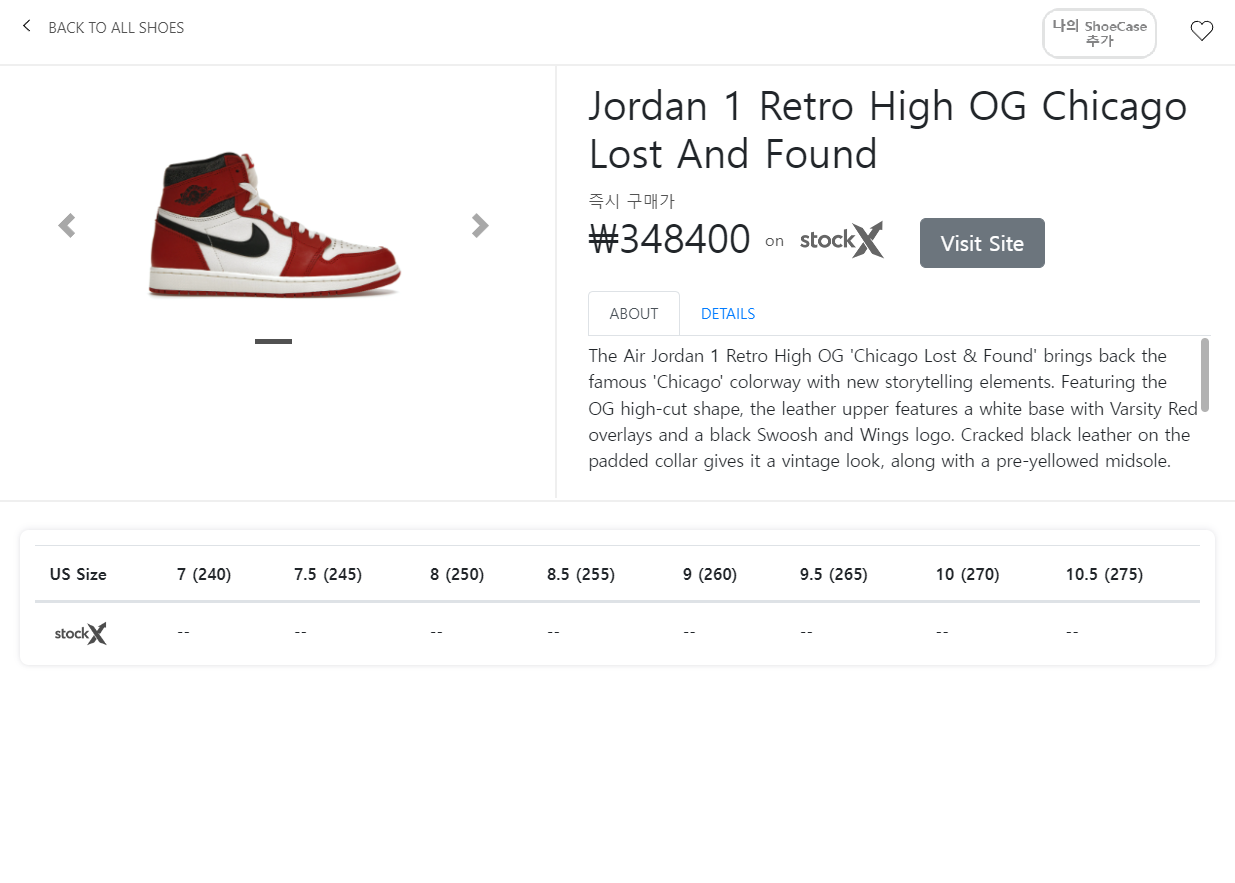
\includegraphics[scale=0.35]{pics/search_detail.png}}
\\When the user clicks the image of the shoes in the search result, a pop-up window appears. The pop-up contains the price of shoes and information about shoes. Also, unlike the pop-up of "Trending Now," the user can add the shoes to the user's shoecase on this pop-up page. \\
	\item Navigation Bar \\
	\begin{enumerate}
		\item[-]Login Button \\\\
		If the user clicks this "Login" button,login pop-up appears.\\
	\end{enumerate}
	\begin{enumerate}
		\item[-]Register Button \\\\
		If the user clicks this "Register" button, registration pop-up appears.\\
	\end{enumerate}
	\begin{enumerate}
		\item[-]Home Button \\\\
		If the user clicks this "Home" button, it goes to the first page of main page.\\
	\end{enumerate}
	\begin{enumerate}
		\item[-]Finding User Button \\\\
		If the user clicks this "Finding User Button" button, it goes to the finding other user page.\\
	\end{enumerate}
	\begin{enumerate}
		\item[-]About Button \\\\
		If the user clicks this "About" button, it goes to the detailed description of this web.\\
	\end{enumerate}

\end{enumerate}

\subsection{My ShoeCase}
When the user presses the "My Shocase" button on the upper right of "Trending Now" on the main page, it switches to its own Shocase screen. Users can add shoes searched on the Search bar to My shoecase, and the added shoes are displayed on this screen. In My Shocase, you can check the price of registered shoes and check the environment for shoe management, such as the temperature and humidity of the shoecase where the shoes are stored.\\\\
\begin{enumerate}
	\item Register Shoes\\\\
\\To register your shoes in the ShoeCase, you need to use the search bar to search shoes. If the user finds the shoes that the user want to register, the user can register the shoes through click the "Add to my ShoeCase"button in search shoes pop-up. My Shoecase page display the registered shoes.\\\\
	
	\item Registered Shoes Information\\\\
\\In "Registered Shoes", registered shoes items can be clicked to display shoe information and real-time resell prices. The shoes information appears with the pop-up page.
The information and price of shoes are implemented to be obtained through the Stockx data. The shoes registered by the user can be shared with others.\\\\
	\item Public/Private Setting\\\\
\\Each item property has a check box where you can set public/private. 
If the checkbox is marked, it will be disclosed. If it is checked, it will be closed.\\\\
	\item The number of Kick\\\\
\\Each person's shoes have the ability to press Kick icon. 
If you press the icon, you can register that user's ShoeCase as a favorite.
The number of Kick is also calculated, so you can see how many people like it.\\\\
\end{enumerate}

\subsection{Finding Other User}
\begin{enumerate}
	\item Search Pop-Up page\\\\
\\\centerline{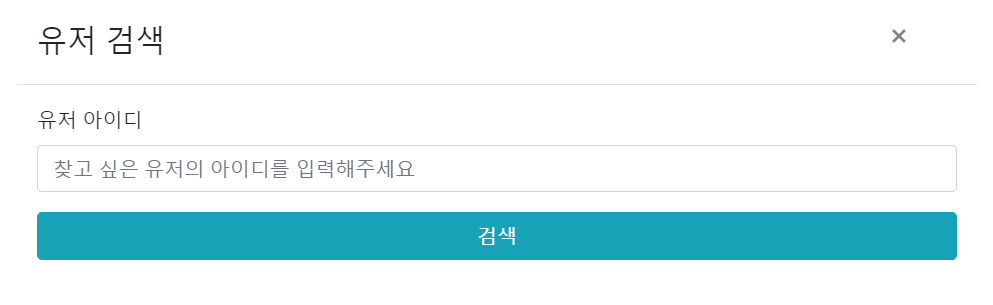
\includegraphics[scale=0.35]{pics/finding_user.png}}\\\\
\\When the user clicks the "Finding Other User" button on the navigation bar at the top of the main page, a pop-up page appears that allows users to search for user names. When the user enters the other user name that the user wants to search in search bar, the user's list corresponding to the word is rendered on the screen.\\\\
	\item Other user's ShoeCase list\\
\\If the user type another user's name in the search box, the shoecases results will be listed.
Clicking on an individual item in the list takes you to the user's individual ShoeCase page depending on whether that is disclosed or not.\\\\
\end{enumerate}

\subsection{Other user's ShoeCase}
\begin{enumerate}
	\item Main ShoeCase Page\\
\\When the user clicks the other user's name searched in "Finding other user", it goes to the user's Shoecase page. Like the "My ShoeCase" page, the user can see the shoes registered by other user.\\\\
	\begin{enumerate}
		\item[-]There is a mark indicating the number of kicks and a "Kick" button that can be pressed. "Kick" is a like button that you can press when you like someone else's ShoeCase. (similar to a heart on Instagram). \\\\
	\end{enumerate}
	\item Detailed ShoeCase Page\\
\\If the user click on the shoes the user want to see the information of the shoes, the pop-up page that has the information of shoes appears. The informations about shoes are the name of the shoes, the real-time present price of shoes from Stockx data.\\
\end{enumerate}
\section{Arcitecture Design and Implementation}
\subsection{Overall Architecture}
\centerline{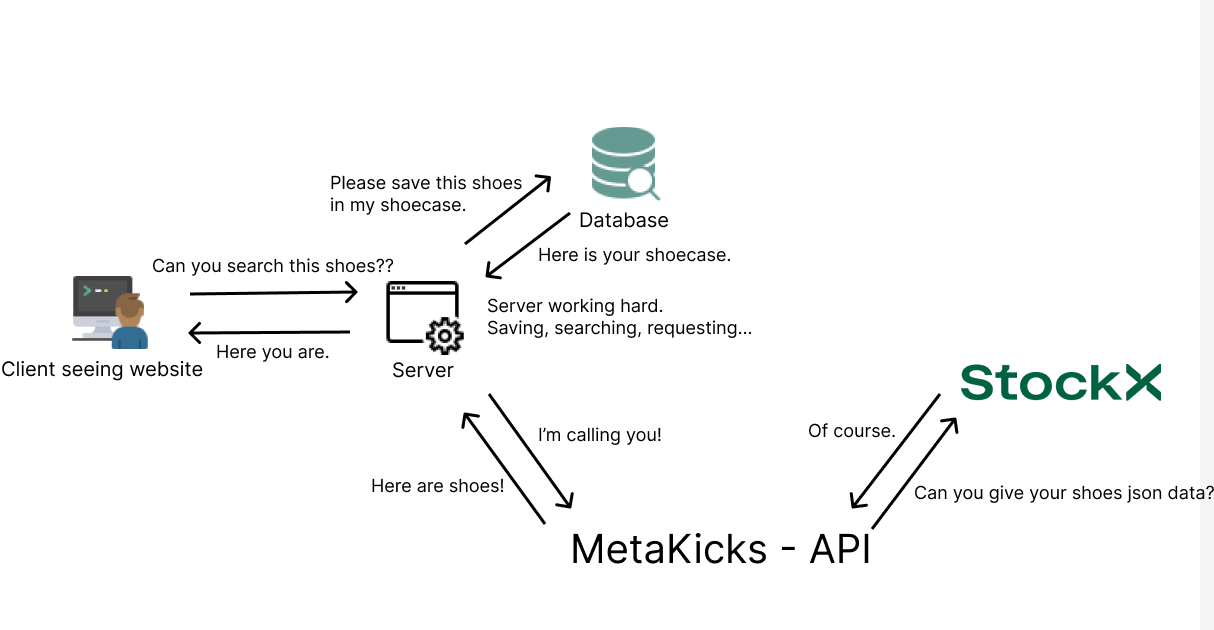
\includegraphics[scale=0.2]{pics/service_construct.png}}
Our MetaKicks site consists of frontend, backend, API, and DB. First, the user registers the shoes in the virtual shoe rack on the frontend page. In this process, users can easily find many kinds of shoes registered on the stockX homepage through API calls through name or style code search. Once you have found the shoes, press the heart button to complete the registration in the database.\\
The front end uses ReactJS to naturally switch the web screen using state. We used Express.js to facilitate the connection with MongoDB, the database we use, and applied stockX API to build a project that calls API when the client requests it from the server.\\
\subsection{Directory Organization}
\begin{table}[h]
\caption{Directory of MetaKicks}
\def\arraystretch{1.24} \small
    \begin{tabular}{|p{2.8cm}|p{2.4cm}|p{2.7cm}|}
        \hline
        \textbf{\textit{Directory}} & \textbf{\textit{File Name}} & \textbf{\textit{Repository}} \\ \hline
        MetaKicks\_Frontend/ & package.json \par package-lock.json \par README.md & MetaKicks\_Frontend\\ \hline
         
        MetaKicks\_Frontend/\par src/ \par & App.css \par App.js \par index.css \par index.js \par serviceWorker.js \par 					setupTests.js \par  & MetaKicks\_Frontend\\ \hline
	
	MetaKicks\_Frontend/\par src/components/ & BrandIcons.js \par FindUserModal.js \par ImgCarousel.js \par MiniCard.js \par NavBar.js \par PriceTable.js \par ProductCard.js \par Products.js \par SearchBar.js \par SignInModal.js \par SignUpModal.js \par Trending.js & MetaKicks\_Frontend\\ \hline
	MetaKicks\_Backend/ & index.js \par package.json \par package-lock.json \par README.md \par & MeatKicks\_Backend\\ \hline
	MetaKicks\_Backend/\par scrapers/ & flightclub-scrape.js \par goat-scraper.js \par stadiumgoods-scraper.js \par stockx-scraper.js & MetaKicks\_Backend\\ \hline
	MetaKicks\_Backend/\par routes/ & routes.js & MetaKicks\_Backend\\ \hline
	MetaKicks\_Backend/\par models & Metakicks.js & MetaKicks\_Backend\\ \hline
	MetaKicks\_Backend/\par controllers & Metakicks.controllers.js & MetaKicks\_Backend\\ \hline
	MetaKicks\_Document/ & MetaKicks.pdf \par MetaKicks.tex \par README.md & MetaKicks\_Document\\ \hline
	\end{tabular}
\end{table}
\subsection{Module 1 : Front End}
\begin{enumerate}
\item Purpose\\
\\\\To develop Metakicks, a platform where the user can see the uesr's and the other's shoecase on the web, we used React, a web framework developed through Javascript language. Since Metakciks is powered on the web, it can be accessed by url without a separate installation. React uses Dirty checking and Virtual DOM to find the DOM element that needs to be updated and only updates that part, so it is possible to perform fast on dynamic webs with frequent re-rendering. Metakicks used React because it is a web that renders only the part without changing the entire page when changing the screen. Also, there is the other advantage. Since React uses javascripts such as node.js and express.js, it has the advantage of using javascript for front-end and back-end development. If the developer knows Javascript, the developer can develop front-end and back-end. Therefore React was adopted as a front-end development environment to enhance the efficiency and develop more efficiently.\\\\
\item Functionality\\
\\\\Metakicks's front-end made with React requests existing JSON file in the database via the backend server to show the users their own shoecase and the other's shoecase. And the information received from the user is delivered to the back-end server and database. With front-end of Metakicks, the user can give their information to the back-end/database and the user can see the data from database with graphic rendering as well as the LG ShoeCase system. Users can get a better experience for Metakicks and LG from innovative idea of Metakicks.\\\\
\item Location of Source Code\\
: MetaKicks\_Frontend/\\\\
\item Class Components\\
	\begin{enumerate}
		\item[-] src/App.js\\\\
		This is the main frame of the main page. This routes to trending now and search result.\\
	\end{enumerate}
	\begin{enumerate}
		\item[-] src/Trending.js\\\\
		Trending screen show the list of products to the screen.Trending screen gets stockX data by requesting to the back-end.\\
	\end{enumerate}
	\begin{enumerate}
		\item[-] src/Products.js\\\\
		Products screen show the list of products of seach result. Products screen gets stockX data by requesting to the back-end.\\
	\end{enumerate}
	\begin{enumerate}
		\item[-] src/Minicard.js\\\\
		Minicard.js turns the list of products into graphic product card.\\
	\end{enumerate}
	\begin{enumerate}
		\item[-] src/ProductCard.js\\\\
		Product Card screen show the detail information and price of shoes.Product Card screen gets stockX data by requesting to the back-end. \\
	\end{enumerate}
\item Where it's taken from\\

\item How and Why We Used It\\

\end{enumerate}
\subsection{Module 2 : Back End}
\begin{enumerate}
\item Purpose\\

\item Functionality\\

\item Location of Source Code\\

\item Class Components\\

\item Where it's taken from\\

\item How and Why We Used It\\

\end{enumerate}
\subsection{Module 3 : Database}
\begin{enumerate}
\item Purpose\\

\item Functionality\\

\item Location of Source Code\\

\item Class Components\\

\item Where it's taken from\\

\item How and Why We Used It\\

\end{enumerate}
\end{document}